% !TEX root = Projektdokumentation.tex
\section{Anhang}

\subsection{Detaillierte Zeitplanung}
\label{app:Zeitplanung}

\tabelleAnhang{ZeitplanungKomplett}

\subsection{Lastenheft (Auszug)}
\label{app:Lastenheft}
Es folgt ein Auszug aus dem Lastenheft mit Fokus auf die Anforderungen:

Die Anwendung muss folgende Anforderungen erfüllen: 
\begin{enumerate}[itemsep=0em,partopsep=0em,parsep=0em,topsep=0em]
\item Benutzeroberfläche (\ac{GUI})
	\begin{enumerate}
	\item Die Webanwendung muss über ein \ac{GUI} verfügen, über das sich sowohl 
    Werber, als auch Geworbene mit ihrer Email-Adresse
    registrieren können.
	\item Das Design des \ac{GUI} soll schlicht und modern gehalten werden.
        \item Außerdem soll es einen Mitarbeiterbereich mit Login geben,
        in dem Mitarbeiter die Möglichkeit haben den \ac{QR}-Code von Gutscheinen
        zu scannen und die Gültigkeit zu überprüfen, sowie den Gutschein zu entwerten.
	\end{enumerate}
\item Responsives Design
	\begin{enumerate}
	\item Die Webanwendung soll in allen gängigen Browsern funktionieren.
        \item Sie soll auf Monitoren aller Größen über den PC nutzbar sein.
        \item Außerdem soll sie über mobile Geräte nutzbar sein.
	\end{enumerate}
\item Sicherheit und Datenschutz
	\begin{enumerate}
        \item Die Kundendaten (Email-Adresse) sollen in verschlüsselter Form
        in der Datenbank gespeichert werden, um sensible Daten zusätzlich zu 
        schützen
        \item Die Datenübertragungen sollen mit \ac{TLS} gesichert sein.
        \item Die \ac{DSGVO} Konformität soll gewährleistet sein.
	\end{enumerate}
\item Automatische Affiliate-Link / Gutscheinerzeugung und Versand (Backend)
        \begin{enumerate}
            \item Bei Registrierung eines Werbers per Email-Adresse soll dieser 
            automatisch einen Affiliate-Link zugesandt bekommen, welcher mit seiner
            user\_id in der Datenbank assoziiert ist.
            \item Registriert sich ein Geworbener durch Aufruf des Affiliate-Links eines Werbers, soll dem Geworbenen ein Affiliate-Link und ein Gutschein
            im \ac{PDF}-Format, inklusive \ac{QR}-Code zum Einlösen des Gutscheins, 
            automatisch zugesandt werden. 
            \item Wird der Gutschein eines Geworbenen von einem Mitarbeiter durch Scannen des \ac{QR}-Codes auf dem Gutschein eingelöst, soll dem Werber ebenfalls ein Gutschein im \ac{PDF}-Format erzeugt und zugesandt werden.
        \end{enumerate}
\end{enumerate}
\newpage
% \subsection{Pflichtenheft (Auszug)}
\label{app:Pflichtenheft}

\subsubsection*{Zielbestimmung}

\begin{enumerate}[itemsep=0em,partopsep=0em,parsep=0em,topsep=0em]
\item Musskriterien % Wikipedia: für das Produkt unabdingbare Leistungen, die in jedem Fall erfüllt werden müssen
	\begin{enumerate}
	\item Modul-Liste: Zeigt eine filterbare Liste der Module mit den dazugehörigen Kerninformationen sowie Symbolen zur Einhaltung des Entwicklungsprozesses an
		\begin{itemize}
		\item In der Liste wird der Name, die Bibliothek und Daten zum Source und Kompilat eines Moduls angezeigt.
		\item Ebenfalls wird der Status des Moduls hinsichtlich Source und Kompilat angezeigt. Dazu gibt es unterschiedliche Status-Zeichen, welche symbolisieren in wie weit der Entwicklungsprozess eingehalten wurde \bzw welche Schritte als nächstes getan werden müssen. So gibt es \zB Zeichen für das Einhalten oder Verletzen des Prozesses oder den Hinweis auf den nächsten zu tätigenden Schritt. 
		\item Weiterhin werden die Benutzer und Zeitpunkte der aktuellen Version der Sourcen und Kompilate angezeigt. Dazu kann vorher ausgewählt werden, von welcher Umgebung diese Daten gelesen werden sollen. 
		\item Es kann eine Filterung nach allen angezeigten Daten vorgenommen werden. Die Daten zu den Sourcen sind historisiert. Durch die Filterung ist es möglich, auch Module zu finden, die in der Zwischenzeit schon von einem anderen Benutzer editiert wurden.
		\end{itemize}
	\item Tag-Liste: Bietet die Möglichkeit die Module anhand von Tags zu filtern. 
		\begin{itemize}
		\item Es sollen die Tags angezeigt werden, nach denen bereits gefiltert wird und die, die noch der Filterung hinzugefügt werden könnten, ohne dass die Ergebnisliste leer wird.
		\item Zusätzlich sollen die Module angezeigt werden, die den Filterkriterien entsprechen. Sollten die Filterkriterien leer sein, werden nur die Module angezeigt, welche mit einem Tag versehen sind.
		\end{itemize}
	\item Import der Moduldaten aus einer bereitgestellten \acs{CSV}-Datei
		\begin{itemize}
		\item Es wird täglich eine Datei mit den Daten der aktuellen Module erstellt. Diese Datei wird (durch einen Cronjob) automatisch nachts importiert.
		\item Dabei wird für jedes importierte Modul ein Zeitstempel aktualisiert, damit festgestellt werden kann, wenn ein Modul gelöscht wurde.
		\item Die Datei enthält die Namen der Umgebung, der Bibliothek und des Moduls, den Programmtyp, den Benutzer und Zeitpunkt des Sourcecodes sowie des Kompilats und den Hash des Sourcecodes.
		\item Sollte sich ein Modul verändert haben, werden die entsprechenden Daten in der Datenbank aktualisiert. Die Veränderungen am Source werden dabei aber nicht ersetzt, sondern historisiert.
		\end{itemize}
	\item Import der Informationen aus \ac{SVN}. Durch einen \gqq{post-commit-hook} wird nach jedem Einchecken eines Moduls ein \acs{PHP}-Script auf der Konsole aufgerufen, welches die Informationen, die vom \ac{SVN}-Kommandozeilentool geliefert werden, an \acs{NatInfo} übergibt.
	\item Parsen der Sourcen
		\begin{itemize}
		\item Die Sourcen der Entwicklungsumgebung werden nach Tags, Links zu Artikeln im Wiki und Programmbeschreibungen durchsucht.
		\item Diese Daten werden dann entsprechend angelegt, aktualisiert oder nicht mehr gesetzte Tags/Wikiartikel entfernt.
		\end{itemize}
	\item Sonstiges
		\begin{itemize}
		\item Das Programm läuft als Webanwendung im Intranet.
		\item Die Anwendung soll möglichst leicht erweiterbar sein und auch von anderen Entwicklungsprozessen ausgehen können.
		\item Eine Konfiguration soll möglichst in zentralen Konfigurationsdateien erfolgen.
		\end{itemize}
	\end{enumerate}
\end{enumerate}

\subsubsection*{Produkteinsatz}

\begin{enumerate}[itemsep=0em,partopsep=0em,parsep=0em,topsep=0em]
\item{Anwendungsbereiche\\
Die Webanwendung dient als Anlaufstelle für die Entwicklung. Dort sind alle Informationen für die Module an einer Stelle gesammelt. Vorher getrennte Anwendungen werden ersetzt \bzw verlinkt.}
\item{Zielgruppen\\
\NI wird lediglich von den \ac{Natural}-Entwicklern in der EDV-Abteilung genutzt.}
\item{Betriebsbedingungen\\ % Wikipedia: physikalische Umgebung des Systems, tägliche Betriebszeit, ständige Beobachtung des Systems durch Bediener oder unbeaufsichtigter Betrieb
Die nötigen Betriebsbedingungen, also der Webserver, die Datenbank, die Versionsverwaltung, das Wiki und der nächtliche Export sind bereits vorhanden und konfiguriert. Durch einen täglichen Cronjob werden entsprechende Daten aktualisiert, die Webanwendung ist jederzeit aus dem Intranet heraus erreichbar.}
\end{enumerate}


% \clearpage
\subsection{Use Case-Diagramm}
\label{app:UseCase}
% Use Case-Diagramme und weitere \acs{UML}-Diagramme kann man auch direkt mit \LaTeX{} zeichnen, siehe \zB \url{http://metauml.sourceforge.net/old/usecase-diagram.html}.
\begin{figure}[htb]

\vspace{7pt}
\begin{center}
\begin{tikzpicture}[
  font=\sffamily\itshape\fontsize{13}{15}\selectfont,
  actor/.style={draw, minimum size=1cm},
  include/.style={dashed,->,>=Latex, line width=1pt},
  extend/.style={dashed,->,>=Latex, line width=1pt},
  note/.style={
    draw,
    fill=yellow!20,
    font=\scriptsize,
    align=left,
    inner sep=3pt,
    rectangle,
    minimum width=2.7cm,
    minimum height=1.7cm,
    path picture={
      % gefaltete Ecke oben links (IHK-konform)
      \draw (path picture bounding box.north west) ++(0.4,0)
        -- ++(0,-0.4) -- (path picture bounding box.north west) -- cycle;
    }
  }
]

    % Funktion zum Zeichnen eines Strichmännchens
    \newcommand{\actor}[3]{%
        % Kopf
        \draw (#1,#2) circle (0.3);
        % Körper
        \draw (#1,#2-0.3) -- (#1,#2-1);
        % Arme
        \draw (#1-0.5,#2-0.6) -- (#1+0.5,#2-0.6);
        % Beine
        \draw (#1,#2-1) -- (#1-0.5,#2-1.5);
        \draw (#1,#2-1) -- (#1+0.5,#2-1.5);
        % Name
        \node[below=1.7cm] at (#1,#2) {#3};
    }

    % Systemgrenze
    \draw[thick, fill=yellow!10]
        (-7,-12.1) rectangle (3,5)
        node[above,xshift=-5cm, yshift=-0.8cm, fill=yellow!25] {Empfehlungsmarketing-App};

    % Akteure
    \actor{-8.5}{3}{Werber}
    \actor{-8.5}{0}{Geworbener}
    \actor{4.5}{3}{Mitarbeiter}

    % Use Cases
    \node[draw, ellipse, fill=yellow!50, minimum height=1cm, minimum width=3cm,
    text width=5cm, align=center] (ucLogin) at (-2,3.0) {Einloggen in Mitarbeiterbereich};

    \node[draw, ellipse, fill=yellow!50, minimum height=1cm, minimum width=1cm,
    text width=3cm, align=center] (ucScan) at (-4.5,0.0) {Gutschein scannen};

    \node[draw, ellipse, fill=yellow!50, minimum height=1cm, minimum width=1cm,
    text width=3cm, align=center] (ucRedeem) at (0.5,0.0) {Gutschein entwerten};

    \node[draw, ellipse, fill=yellow!50, minimum height=1cm, minimum width=3cm,
    text width=2.5cm, align=center] (ucAffLink) at (-4.7,-6.5) {Affiliate-Link senden};

    \node[draw, ellipse, fill=yellow!50, minimum height=1cm, minimum width=3cm,
    text width=2cm, align=center] (ucVoucherSend) at (1.0,-6.5) {Gutschein senden};

    \node[draw, ellipse, fill=yellow!50, minimum height=1cm, minimum width=3cm,
    text width=5cm, align=center] (ucRegister) at (-2,-9.4) {Registrieren mit Email-Adresse};

    % Verbindungen zu Akteuren
    \draw (-7.5,2.0) -- (ucRegister.west);
    \draw (-7.5,-0.5) -- (ucRegister.west);
    \draw (4,2.2) -- (ucRedeem.east);
    \draw (4,2.2) -- (ucScan.east);
    \draw (4,2.2) -- (ucLogin.east);

    % <<include>>: Gutscheinprüfung benötigt Login
    \draw[include] (ucRedeem.north) --
      node[right,sloped,above]{\fontsize{11}{13}\selectfont\bfseries <<include>>}
      (ucLogin.south);
    \draw[include] (ucScan.north) --
      node[right,sloped,above]{\fontsize{11}{13}\selectfont\bfseries <<include>>}
      (ucLogin.south);

    % <<include>>: Registrierung umfasst immer Affiliate-Link und optional Gutschein senden
    \draw[include] (ucAffLink.south) --
      node[right,sloped,above]{\fontsize{11}{13}\selectfont\bfseries <<include>>}
      (ucRegister.north);
    \draw[extend] (ucVoucherSend.south) --
      node[left,sloped,above]{\fontsize{11}{13}\selectfont\bfseries <<extend>>}
      (ucRegister.north);

    % <<extend>>: Gutschein einlösen -> Werber erhält Gutschein
    \draw[extend] (ucVoucherSend.north) -- (ucRedeem.south)
      node[midway,sloped,above]{\fontsize{11}{13}\selectfont\bfseries <<extend>>};

    % UML-Notiz (IHK-konform, Ecke oben links), an die Beziehung gehängt
    \node[note] (note1) at (-4,-2.0) {Bedingung:\\ Gutschein entwertet};
    \draw[dashed] (note1.east) -- ++(0,0) |- ($(ucVoucherSend.north)!0.75!(ucRedeem.south)$);

    \node[note] (note2) at (-2,-4.5) {Bedingung:\\ Registrierung über\\ Affiliate-Link};
    \draw[dashed] (note2.south) -- ++(0,0) |- ($(ucVoucherSend.south)!0.05!(ucRegister.north)$);

    % ===== Legende unten rechts =====
    \node[draw, fill=yellow!20, align=left, font=\scriptsize, anchor=north east] at (3,-10.3) (legend) {
        \textbf{Legende}\\[3pt]
        \begin{tabular}{@{}ll@{}}
          \raisebox{0.5ex}{\tikz{\draw[dashed,->,>=Latex,line width=1pt] (0,0)--(0.8,0);}} & <<include>> = verpflichtender Use Case \\[6pt]
          \raisebox{0.5ex}{\tikz{\draw[dashed,->,>=Latex,line width=1pt] (0,0)--(0.8,0);}} & <<extend>> = optionaler Use Case \\
        \end{tabular}
    };

\end{tikzpicture}
\end{center}

% \includegraphicsKeepAspectRatio{UseCase.pdf}{0.7}
\caption{Use Case-Diagramm}
\end{figure}


\newpage
\subsection{Datenbankmodell}
\label{app:Datenbankmodell}
\begin{figure}[h]
\centering
\begin{tikzpicture}[
  font=\sffamily\small,
  >=Latex,
  node distance=18mm and 24mm,
  entity/.style={
    draw,
    rounded corners,
    fill=blue!5,
    align=left,
    inner sep=3.5mm,
    minimum width=4.4cm,
    text depth=0pt
  },
  rel/.style={-Latex, thick},
  card/.style={midway, fill=white, inner sep=1pt}
]

% --- Entities ---------------------------------------------------
\node[entity] (users) {\textbf{users}\\
  \pk{id (PK)}\\
  \attr{email\_enc}\\
  \attr{email\_iv}\\
  \attr{email\_tag}\\
  \attr{email\_hash}\\
  \attr{referral\_code}\\
  \fk{referrer\_id (FK)}\\
  \attr{created\_at}
};

\node[entity, right=of users] (vouchers) {\textbf{vouchers}\\
  \pk{id (PK)}\\
  \fk{user\_id (FK)}\\
  \attr{code}\\
  \attr{discount\_percent}\\
  \attr{expires\_at}\\
  \attr{created\_at}
};

\node[entity, below=of vouchers] (redemptions) {\textbf{redemptions}\\
  \pk{id (PK)}\\
  \fk{voucher\_id (FK)}\\
  \fk{employee\_id (FK)}\\
  \attr{redeemed\_at}
};

\node[entity, below=of users] (maillog) {\textbf{mail\_log}\\
  \pk{id (PK)}\\
  \fk{to\_user\_id (FK)}\\
  \attr{subject}\\
  \attr{success}\\
  \attr{error}\\
  \attr{created\_at}
};

\node[entity, below=of redemptions] (employees) {\textbf{employees}\\
  \pk{id (PK)}\\
  \attr{first\_name}\\
  \attr{last\_name}\\
  \attr{email}\\
  \attr{created\_at}
};

% --- Relationships ----------------------------------------------
\draw[rel] (users) -- 
  node[card, xshift=-20pt] {1} 
  node[card, pos=0.8, xshift=-2pt] {N} 
  (vouchers);

\draw[rel] (vouchers) -- 
  node[card, xshift=7pt, yshift=15] {1} 
  node[card, pos=0.8, xshift=7pt, yshift=3] {1} 
  (redemptions);

\draw[rel] (employees) -- 
  node[card, xshift=7pt, yshift=-13] {1} 
  node[card, pos=0.8, xshift=7pt, yshift=-1] {N} 
  (redemptions);

\draw[rel] (users) -- 
  node[card, xshift=7pt, yshift=13] {1} 
  node[card, pos=0.8, xshift=7pt, yshift=0] {N} 
  (maillog);
\end{tikzpicture}
\caption{Vereinfachtes Datenbankschema (MySQL)}


% \includegraphicsKeepAspectRatio{database.pdf}{1}
% \caption{Datenbankmodell}
\end{figure}

\newpage
\subsection{Screenshots der Anwendung}
\label{sec:screenshots}
\subsubsection{Registrierungsformular}
\begin{figure}[H]
    \centering
    
\includegraphics[width=0.8\linewidth]{Bilder/screenshots/form_blank.png}
    \caption{Leeres Formular}
    \label{fig:placeholder}
\end{figure}

\begin{figure}[H]
    \centering
    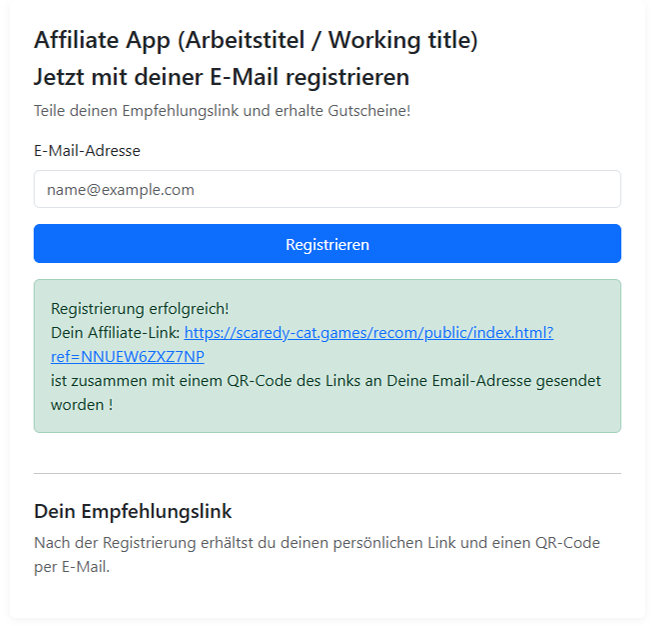
\includegraphics[width=0.8\linewidth]{Bilder/screenshots/form_registered.png}
    \caption{Erfolgreiche Registrierung}
    \label{fig:placeholder}
\end{figure}

\begin{figure}[H]
    \centering
    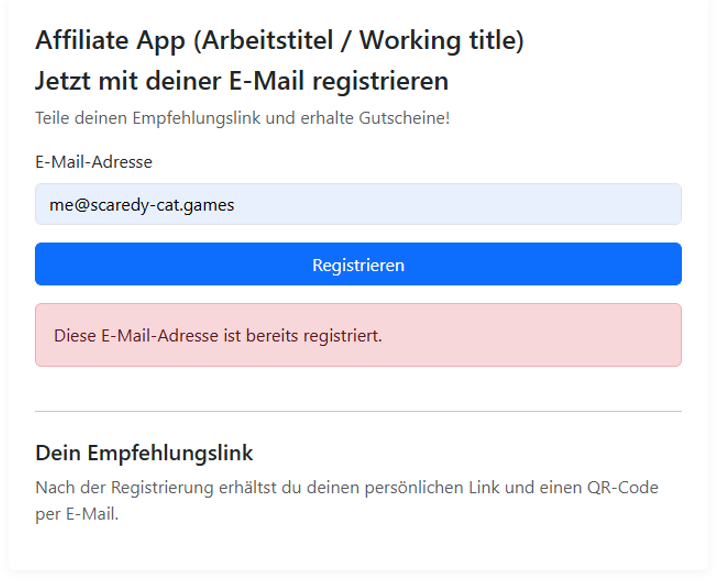
\includegraphics[width=0.8\linewidth]{Bilder/screenshots/form_already_registered.png}
    \caption{Fehlermeldung bei doppeltem Registrierungsversuch}
    \label{fig:placeholder}
\end{figure}

\subsubsection{Emails an Werber oder Geworbenen}
\begin{figure}[H]
    \centering
    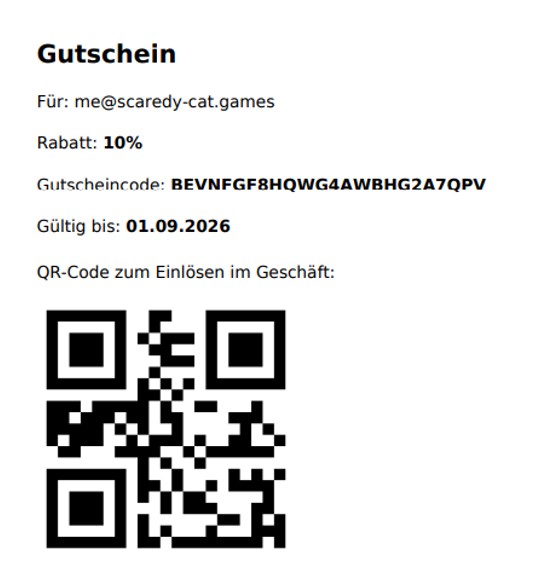
\includegraphics[width=0.5\linewidth]{Bilder/screenshots/email_voucher.png}
    \caption{Gutschein an Werber/Geworbenen}
    \label{fig:placeholder}
\end{figure}

\begin{figure}[H]
    \centering
    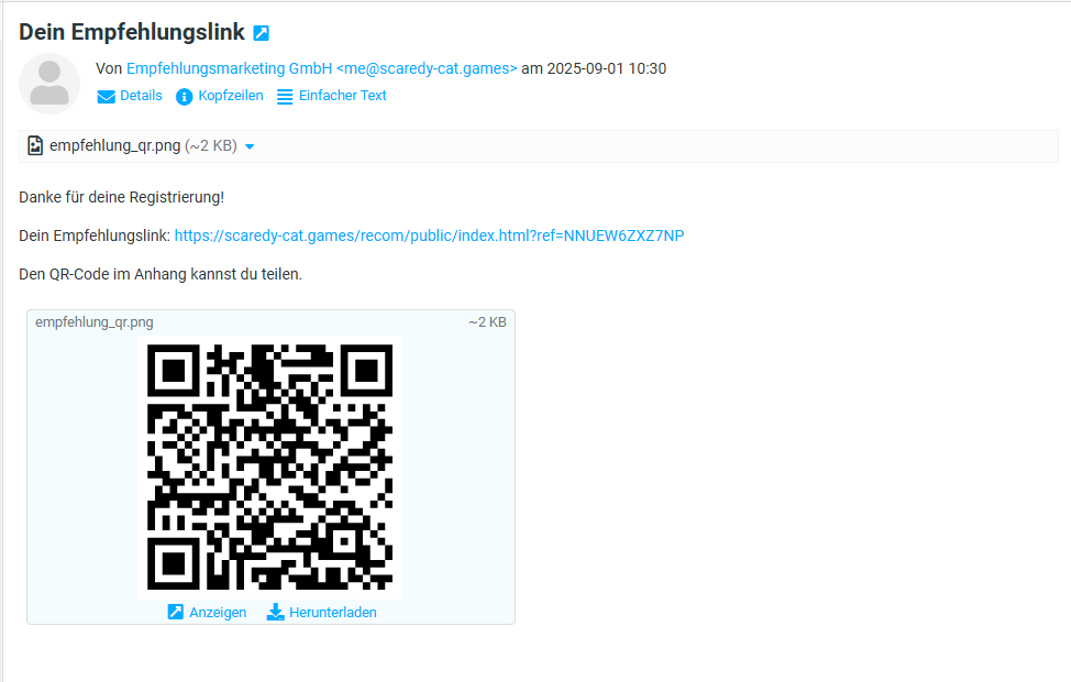
\includegraphics[width=1.0\linewidth]{Bilder/screenshots/mail_affiliate_link.png}
    \caption{Affiliate-Link und QR-Code an Werber/Geworbenen}
    \label{fig:placeholder}
\end{figure}



% \subsection{Oberflächenentwürfe}
\label{app:Entwuerfe}
\begin{figure}[htb]
\centering
\includegraphicsKeepAspectRatio{MockupModules.pdf}{0.7}
\caption{Liste der Module mit Filtermöglichkeiten}
\end{figure}

\begin{figure}[htb]
\centering
\includegraphicsKeepAspectRatio{MockupModul.pdf}{0.7}
\caption{Anzeige der Übersichtsseite einzelner Module}
\end{figure}

\begin{figure}[htb]
\centering
\includegraphicsKeepAspectRatio{MockupTag.pdf}{0.7}
\caption{Anzeige und Filterung der Module nach Tags}
\end{figure}

% \clearpage
% \subsection{Screenshots der Anwendung}
\label{Screenshots}
\begin{figure}[htb]
\centering
\includegraphicsKeepAspectRatio{tagliste.pdf}{1}
\caption{Anzeige und Filterung der Module nach Tags}
\end{figure}
\clearpage
\begin{figure}[htb]
\centering
\includegraphicsKeepAspectRatio{modulliste.pdf}{1}
\caption{Liste der Module mit Filtermöglichkeiten}
\end{figure}
\clearpage

% \subsection{Entwicklerdokumentation}
\label{app:Doc}
\begin{center}
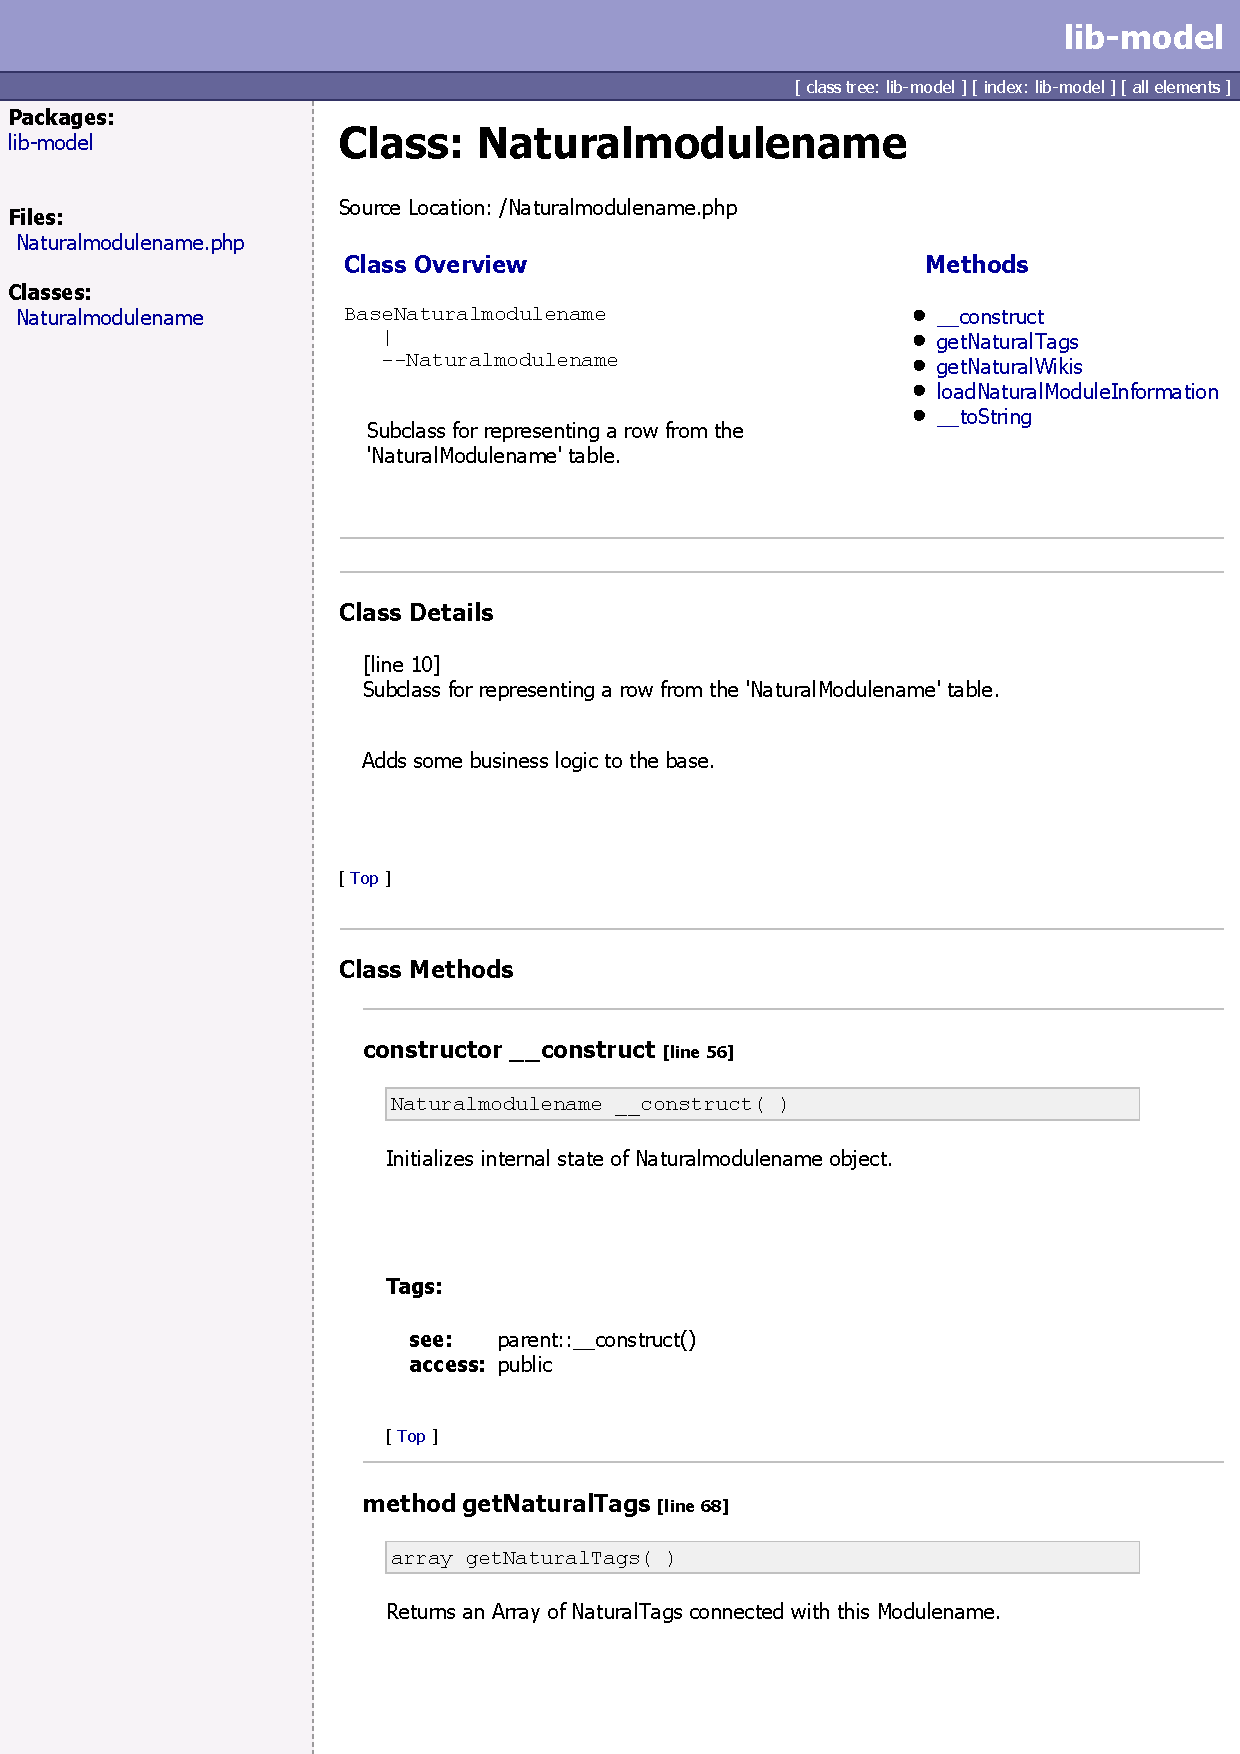
\includegraphics[page=1, width=0.9\textwidth]{doc.pdf}

\includegraphics[page=2, width=0.9\textwidth]{doc.pdf}
\end{center}

% \clearpage
% \subsection{Testfall und sein Aufruf auf der Konsole}
\label{app:Test}
\lstinputlisting[language=php, caption={Testfall in PHP}]{Listings/tests.php}
\clearpage
\begin{figure}[htb]
\centering
\includegraphicsKeepAspectRatio{testcase.jpg}{1}
\caption{Aufruf des Testfalls auf der Konsole}
\end{figure}


% \subsection{Klasse: ComparedNaturalModuleInformation}
% \label{app:CNMI}
% Kommentare und simple Getter/Setter werden nicht angezeigt.
% \lstinputlisting[language=php, caption={Klasse: ComparedNaturalModuleInformation}]{Listings/cnmi.php}
% \clearpage

% \subsection{Klassendiagramm}
% \label{app:Klassendiagramm}
% Klassendiagramme und weitere \acs{UML}-Diagramme kann man auch direkt mit \LaTeX{} zeichnen, siehe \zB \url{http://metauml.sourceforge.net/old/class-diagram.html}.
% \begin{figure}[htb]
% \centering
% \includegraphicsKeepAspectRatio{Klassendiagramm.pdf}{1}
% \caption{Klassendiagramm}
% \end{figure}
% \clearpage

% \subsection{Benutzerdokumentation}
\label{app:BenutzerDoku}
Ausschnitt aus der Benutzerdokumentation:

\begin{table}[htb]
\begin{tabularx}{\textwidth}{cXX}
\rowcolor{heading}\textbf{Symbol} & \textbf{Bedeutung global} & \textbf{Bedeutung einzeln} \\
\includegraphicstotab[]{weather-clear.png} & Alle Module weisen den gleichen Stand auf. & Das Modul ist auf dem gleichen Stand wie das Modul auf der vorherigen Umgebung. \\
\rowcolor{odd}\includegraphicstotab[]{weather-clear-night.png} & Es existieren keine Module (fachlich nicht möglich). & Weder auf der aktuellen noch auf der vorherigen Umgebung sind Module angelegt. Es kann also auch nichts übertragen werden. \\
\includegraphicstotab[]{weather-few-clouds-night.png} & Ein Modul muss durch das Übertragen von der vorherigen Umgebung erstellt werden. & Das Modul der vorherigen Umgebung kann übertragen werden, auf dieser Umgebung ist noch kein Modul vorhanden. \\
\rowcolor{odd}\includegraphicstotab[]{weather-few-clouds.png} & Auf einer vorherigen Umgebung gibt es ein Modul, welches übertragen werden kann, um das nächste zu aktualisieren. & Das Modul der vorherigen Umgebung kann übertragen werden um dieses zu aktualisieren. \\
\includegraphicstotab[]{weather-storm.png} & Ein Modul auf einer Umgebung wurde entgegen des Entwicklungsprozesses gespeichert. & Das aktuelle Modul ist neuer als das Modul auf der vorherigen Umgebung oder die vorherige Umgebung wurde übersprungen. \\
\end{tabularx}
\end{table}


